Das CRISP-DM Modell (Cross-Industry Standard Process for Data Mining) ist ein bewährtes und strukturiertes Modell für Data Mining Projekte. 
CRISP-DM wurde 1996 durch ein Konsortium bestehend aus Daimler-Benz, SPSS, NCR und der niederländischen Versicherungsgesellschaft OHRA konzipiert und 2000 in der Version 1.0 veröffentlicht. (vgl. Zitat: "CRISP-DM 1.0: A Standard Process Model for Data Mining", Shearer, C., 2000).
Das Modell hat sich als de facto Standard in der Data Mining Community etabliert und wird laut verschiedenen Umfragen von 2002, 2004, 2007 und 2014 als führende Methodik von Data Mining Experten verwendet. (vgl. Zitat Data Science Central, 2016).

Das Modell unterteilt den Prozess des Data Mining in sechs verschiedene Phasen.

\begin{figure}[ht]
    \centering
    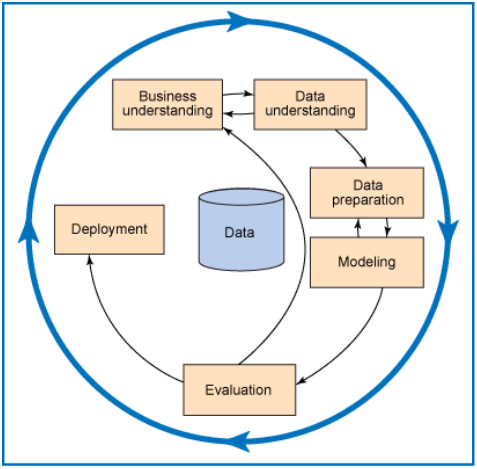
\includegraphics[width=0.7\textwidth]{figures/crispdm.png}
    \caption{Die 6 Phasen des CRISP-DM Modells}
    \label{fig:crispdm}
\end{figure}

Das besondere an diesem Vorgehen ist, dass es an die teils nicht-lineare struktur von KI oder Deep Learning Projekten (vgl. Zitat Data Science Central, 2026) angepasst ist. Auch ein iteratives Vorgehen, welches in solchen Projekten angewendet wird, kann mit dem CRISP-DM Modell abgebildet werden wie auch in der Abbildung \ref{fig:crispdm} zu sehen ist. Das ist wichtig da die Schritte in der Praxis oft nicht linear abgearbeitet werden können und es wichtig ist die Flexibilität zu haben, vorherige Schritte zu wiederholen um deren Resultate zu verbessern oder anzupassen.

Um ein tieferes und besseres Verständnis für die sechs Phasen des CRISP-DM Modells in der Theorie zu bekommen, werden diese im Folgenden genauer beschrieben. In den darauf folgenden Unterkapiteln wird dann erläutert, wie diese Phasen in der Arbeit angewendet werden, um die Forschungsfrage zu beantworten.

\textbf{Business Understanding:}

Der erste Schritt im CRISP-DM-Prozess ist das Business Understanding. Diese Phase bildet die Grundlage des Projekts und fokussiert sich auf das Verständnis der Projektziele und die Anforderungen aus geschäftlicher Perspektive. In dieser Phase werden die Geschäftsziele definiert, die aktuelle Situation bewertet und die analytischen Ziele festgelegt (vgl. Zitat Data Science Central und Zitat PAM Analytics).

\textbf{Data Understanding:}
In der zweiten Phase, der Data Understanding Phase, wird eine erste Datensammlung durchgeführt, um ein erstes Verständnis für die Daten zu bekommen. Diese Phase umfasst die Identifikation relevanter Datenquellen, die Sammlung von Daten und die erste Analyse der Daten, um deren Qualität und Struktur zu bewerten (vgl. Zitat Data Science Central und Zitat PAM Analytics).

\textbf{Data Preparation:}
In der Data Preparation Phase werden die gesammelten Daten aufbereitet und für die Modellierung vorbereitet. Diese Phase umfasst die Bereinigung der Daten, die Transformation der Daten in ein geeignetes Format und die Auswahl relevanter Merkmale (Features) für die Modellierung. Ziel dieser Phase ist es, die Daten in einem Zustand zu bringen, der für die Modellierung geeignet ist (vgl. Zitat Data Science Central und Zitat PAM Analytics).

\textbf{Modeling:}
In der Modeling Phase werden verschiedene Modelle entwickelt und getestet, um die analytischen Ziele zu erreichen. Diese Phase umfasst die Auswahl geeigneter Modellierungstechniken, die Entwicklung von Modellen und die Bewertung der Modelle hinsichtlich ihrer Leistung. Ziel dieser Phase ist es, ein Modell zu entwickeln, das die gestellten Anforderungen erfüllt (vgl. Zitat Data Science Central und Zitat PAM Analytics).

\textbf{Evaluation:}
In der Evaluation Phase werden die entwickelten Modelle bewertet und überprüft, ob sie die gestellten Anforderungen erfüllen. Diese Phase umfasst die Überprüfung der Modellleistung, die Validierung der Modelle und die Entscheidung, ob das Modell in der Praxis eingesetzt werden kann. Ziel dieser Phase ist es, sicherzustellen, dass das entwickelte Modell den geschäftlichen Anforderungen entspricht (vgl. Zitat Data Science Central und Zitat PAM Analytics).

\textbf{Deployment:}
In der letzten Phase, der Deployment Phase, wird das entwickelte Modell in der Praxis eingesetzt. Diese Phase umfasst die Implementierung des Modells, die Überwachung des Modells im Betrieb und die Anpassung des Modells bei Bedarf. Ziel dieser Phase ist es, sicherzustellen, dass das Modell in der Praxis erfolgreich eingesetzt wird und die gewünschten Ergebnisse liefert (vgl. Zitat Data Science Central und Zitat PAM Analytics).